\chapter{Justificación}
\label{cap:justificacion}

\section{Soluciones y alternativas existentes}
\label{sec:alternativas}

Actualmente, en el mercado podemos encontrar diferentes herramientas o programas llamados descompiladores o reversores los cuales tienen la capacidad de convertir un ejecutable
en un código C aproximado llamado normalmente por estas herramiento como pseudocódigo.

Así mismo, la mayoría de estas herramientas están más orientadas a la generación de un código ensamblador más "amigable" y que mayoritariamente siempre necesitara intervención
para que pueda ser más legible y asi ayudar en procesos de depuración.

Algunas de estas herramientas son:

\begin{itemize}
    \item \bf IDA Pro\footnote{Enlace a la página web del producto \href{https://hex-rays.com/ida-pro/}{IDA Pro}}
    \item \bf Ghidra\footnote{Enlace a la página web del producto \href{https://ghidra-sre.org/}{Ghidra}}
    \item \bf AllyDbg\footnote{Enlace a la página web del producto \href{https://www.ollydbg.de/}{AllyDbg}}
\end{itemize}

En la proxima sección detallaremos un poco mas la herramienta IDA Pro en su vertiente gratuita llamda IDA Free\footnote{Enlace a la página web del producto \href{https://hex-rays.com/ida-free/}{IDA Free}},
ya que esta es la más usada para aplicar ingeniería inversa.

\subsection{IDA Pro}
\label{subsec:IDA_pro}

IDA o \textit{Interactive Disassembler} es un desensamblador que es utilizado para ingeniería inversa. IDA soporta una variedad de formato de ejecutables para diferentes procesadores y
sistemas operativos. Tambien es usado como depurador para ejecutables del tipo Windows PE, Mac OS X, Mach-O y Linux ELF\cite{IDAPro_Wikipedia}. Aunque nativamente IDA no teine decompilador, 
en sus ultimas versiones dispones de un \textit{plugin} que nos brinda esta funcionalidad. Cabe destacar que este plugin es un decompilador basado en \textit{cloud}, es decir requiere
de conexión a internet para poder generar un pseudocódigo a partir de un ejecutable.

Para poder analizar en mas profundidad esta herramienta he hecho diferentes pruebas con codigos muy sencillas para poder comprobar que tipo de solucion nos da esta herramienta. Para ello
he utilizado el codigo \ref{cod:binarySearch}, donde se oberva la implementación del algoritmo de busqueda binaria en código C.

\begin{code}
    \begin{minted}{c}
    /** Recursive implementation
    * \param[in] arr array to search
    * \param l left index of search range
    * \param r right index of search range
    * \param x target value to search for
    * \returns location of x assuming array arr[l..r] is present
    * \returns -1 otherwise
    */
    int binarysearch1(const int *arr, int l, int r, int x)
    {
        if (r >= l)
        {
            int mid = l + (r - l) / 2;

            // If element is present at middle
            if (arr[mid] == x)
                return mid;

            // If element is smaller than middle
            if (arr[mid] > x)
                return binarysearch1(arr, l, mid - 1, x);

            // Else element is in right subarray
            return binarysearch1(arr, mid + 1, r, x);
        }

        // When element is not present in array
        return -1;
    }

    /** Iterative implementation
    * \param[in] arr array to search
    * \param l left index of search range
    * \param r right index of search range
    * \param x target value to search for
    * \returns location of x assuming array arr[l..r] is present
    * \returns -1 otherwise
    */
    int binarysearch2(const int *arr, int l, int r, int x)
    {
        int mid = l + (r - l) / 2;

        while (arr[mid] != x)
        {
            if (r <= l || r < 0)
                return -1;

            if (arr[mid] > x)
                // If element is smaller than middle
                r = mid - 1;
            else
                // Else element is in right subarray
                l = mid + 1;

            mid = l + (r - l) / 2;
        }

        // When element is not present in array
        return mid;
    }
    \end{minted}
    \captionof{listing}[Búsqueda binaria, iterativa y recursiva]{Búsqueda binaria, iterativa y recursiva (\cite{BinarySearchGitHub})}
    \label{cod:binarySearch}
\end{code}

Compilamos el código y con el ejecutable que nos genera se lo damos a IDA Free y utilizando el plugin de decompilacor basado en \textit{cloud} generamos un pseudocódigo de los metodos
que encontramos en el código \ref{cod:binarySearch}. En la figura \ref{fig:IDAPro_binaryseacrh1} podemos observar la funcion \textit{binarysearch1()} y en la figura \ref{fig:IDAPro_binaryseacrh2}
podemos observar la funcion \textit{binarysearch2()}.

\begin{figure} [h!]
    \begin{center}
      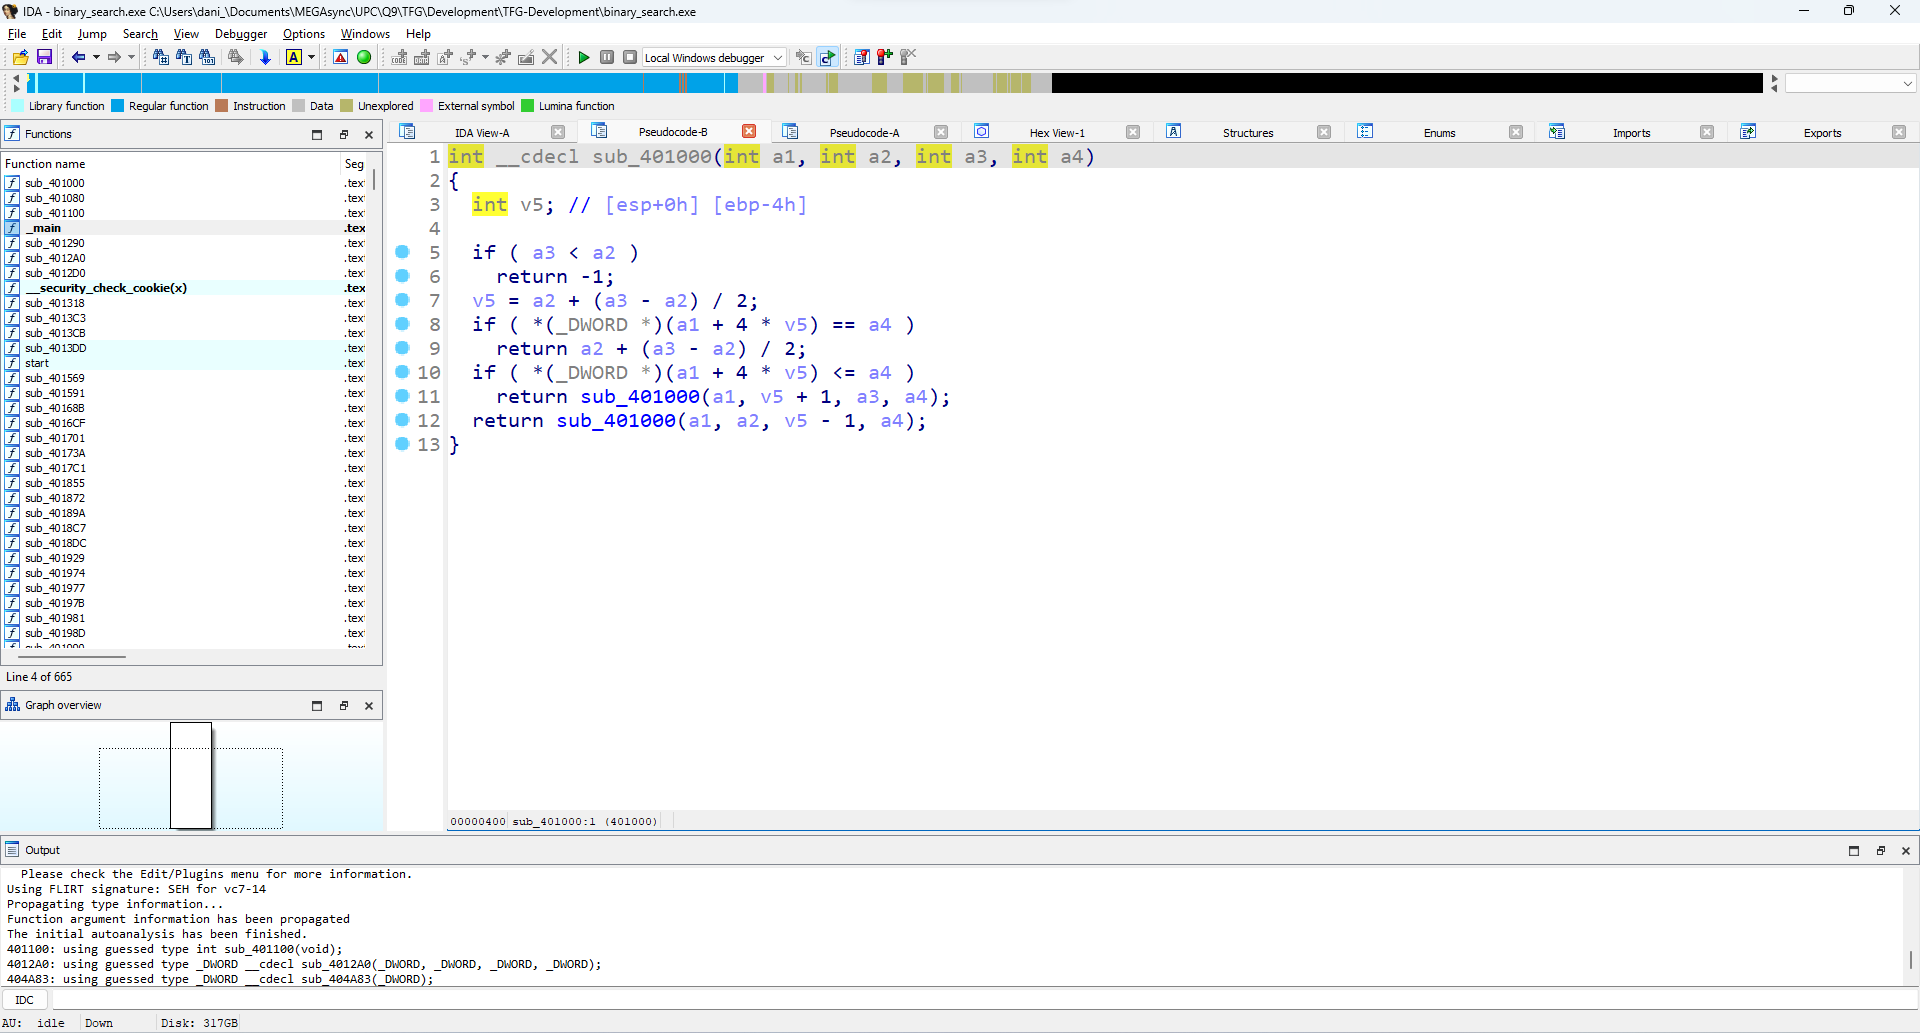
\includegraphics[width=15cm]{figuras/Capitulo_2/Cap_2_IDAPro_binaryseacrh1.png}
    \end{center}
    \caption[Captura de pantalla de IDA Free con el pseudocódigo generado para la funcion \textit{binaryseacrh1}]{Captura de pantalla de IDA Free con el pseudocódigo generado para la funcion \textit{binaryseacrh1} (Elaboración propia)}
    \label{fig:IDAPro_binaryseacrh1}
\end{figure}\

\begin{figure} [h!]
    \begin{center}
      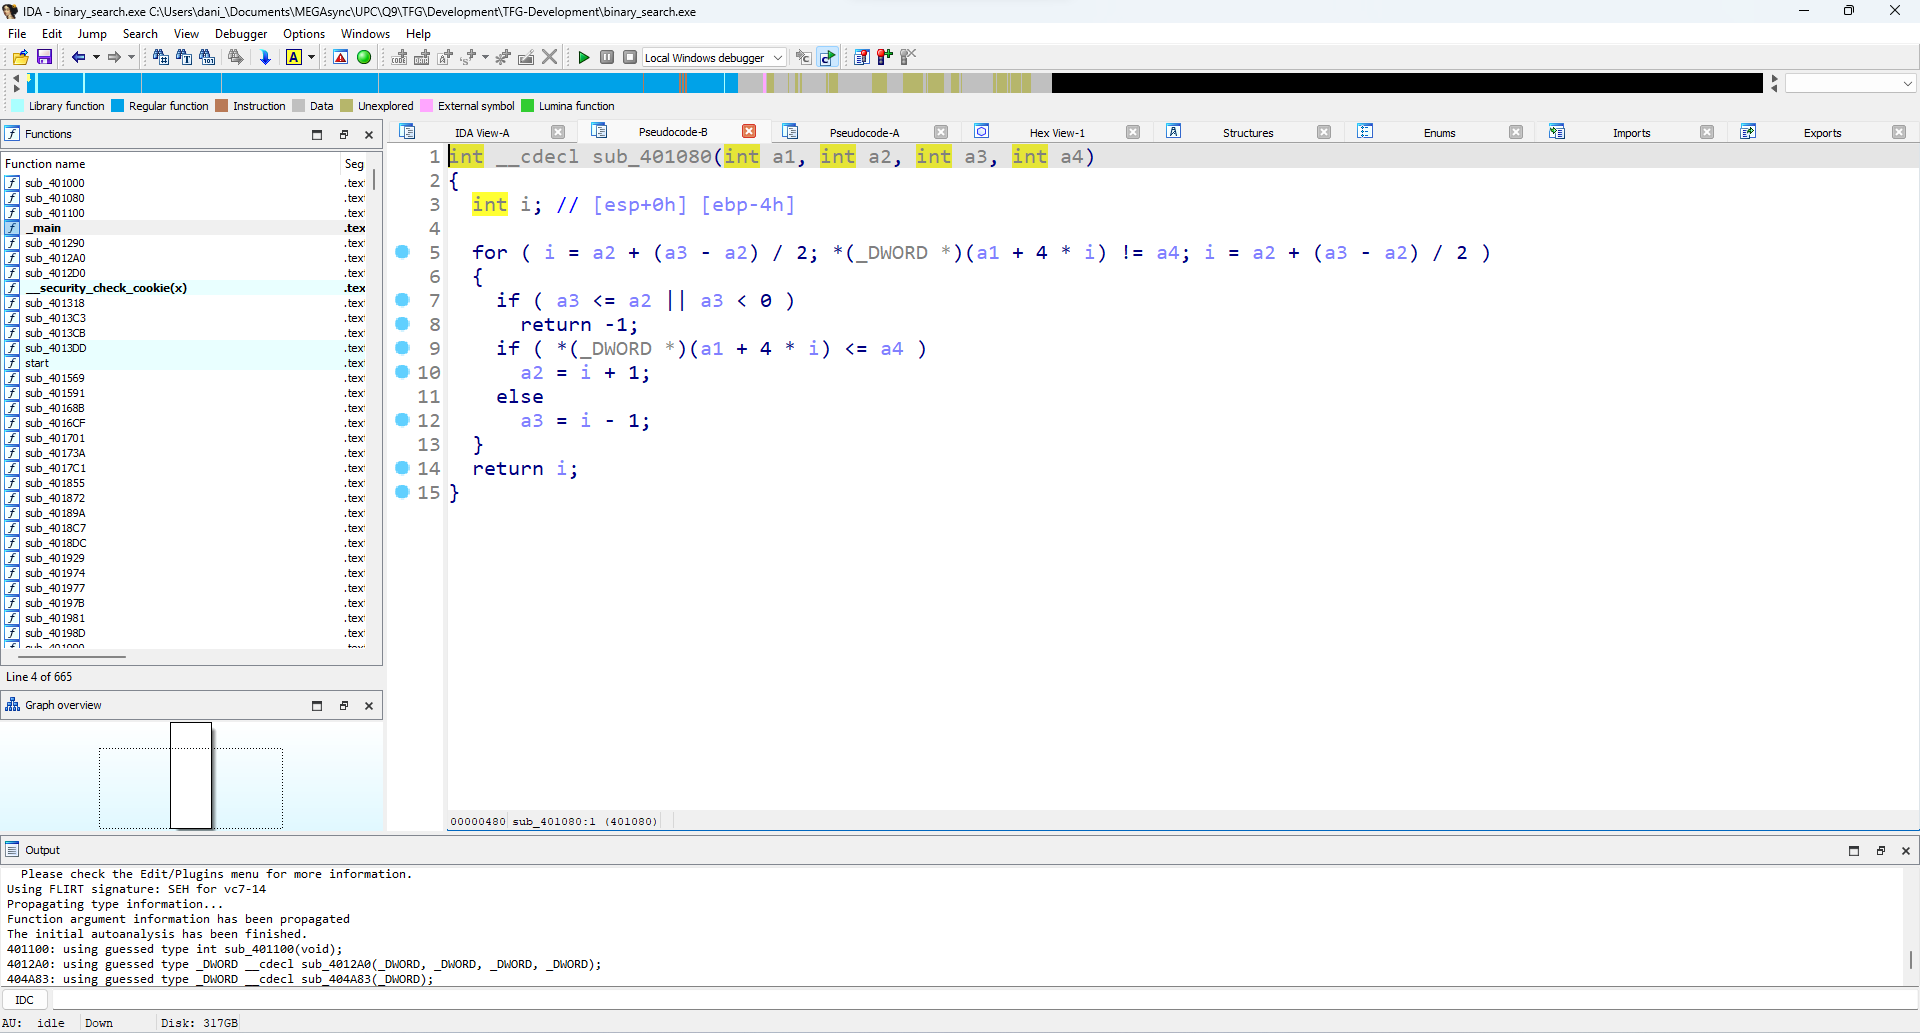
\includegraphics[width=15cm]{figuras/Capitulo_2/Cap_2_IDAPro_binaryseacrh2.png}
    \end{center}
    \caption[Captura de pantalla de IDA Free con el pseudocódigo generado para la funcion \textit{binaryseacrh2}]{Captura de pantalla de IDA Free con el pseudocódigo generado para la funcion \textit{binaryseacrh2} (Elaboración propia)}
    \label{fig:IDAPro_binaryseacrh2}
\end{figure}\

Observamos que el pseudocódigo que nos facilitan se asemeja al codigo original le queda ciertos aspectos en los cuales podria mejorar.

\section{Solucion tomada}
\label{sec:solucion}

% Corregido

La solución tomada pasa por investigar si el uso de inteligencia artificial, más concretamente el uso de modelos de lenguaje preentrenados, nos podría ayudar a la hora de hacer
ingeniería inversa sobre un programa en su forma de ejecutable u objeto.

Para poder hacerlo se decide utilizar modelos de lenguaje disponibles en Internet que la propia comunidad de desarrollo de software libre ha creado o modelos liberados por Microsoft.
La intención es aplicar \textit{fine-tuning} sobre estos modelos ya preentrenados, de tal manera que podemos aumentar la calidad de los resultados obtenidos para nuestra
tarea específica.

Así mismo, se tendrá que investigar sobre que método de \textit{fine-tuning} podemos utilizar, que se ajuste más a la características de nuestra tarea, teniendo en cuenta cosas como el
tipo de datos que se utilizan y el resultado que se quiere obtener.
